% This file was created with tikzplotlib v0.10.1.
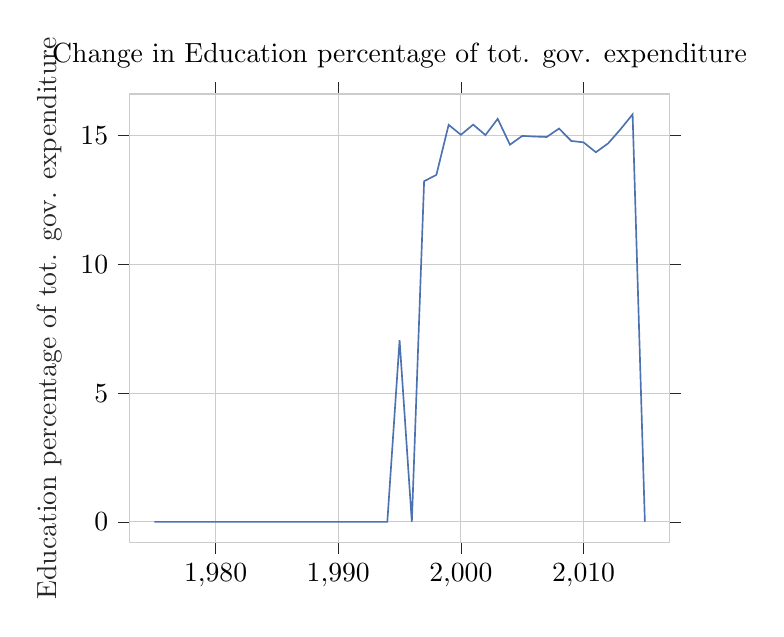
\begin{tikzpicture}

\definecolor{darkslategray38}{RGB}{38,38,38}
\definecolor{lightgray204}{RGB}{204,204,204}
\definecolor{steelblue76114176}{RGB}{76,114,176}

\begin{axis}[
axis line style={lightgray204},
tick align=outside,
title={Change in Education percentage of tot. gov. expenditure},
x grid style={lightgray204},
xmajorgrids,
xmajorticks=true,
xmin=1973, xmax=2017,
xtick style={color=darkslategray38},
y grid style={lightgray204},
ylabel=\textcolor{darkslategray38}{Education percentage of tot. gov. expenditure},
ymajorgrids,
ymajorticks=true,
ymin=-0.790899230769231, ymax=16.6088838461538,
ytick style={color=darkslategray38}
]
\addplot [semithick, steelblue76114176]
table {%
1975 0
1976 0
1977 0
1978 0
1979 0
1980 0
1981 0
1982 0
1983 0
1984 0
1985 0
1986 0
1987 0
1988 0
1989 0
1990 0
1991 0
1992 0
1993 0
1994 0
1995 7.055955
1996 0
1997 13.2223973913043
1998 13.4696782051282
1999 15.410756
2000 15.0253090598291
2001 15.4194506306306
2002 15.0135459504132
2003 15.6432702777778
2004 14.6401925833333
2005 14.9814519266055
2006 14.9566987962963
2007 14.9396314814815
2008 15.2665068907563
2009 14.785587826087
2010 14.7308462295082
2011 14.3476642727273
2012 14.688868172043
2013 15.2306497333333
2014 15.8179846153846
2015 0
};
\end{axis}

\end{tikzpicture}
